%------------------------------------------%
% Cannabis Data Science
% Date: 1/4/2024
%------------------------------------------%
\documentclass[xcolor={dvipsnames}]{beamer}
\hypersetup{pdfpagemode = FullScreen}
\mode<presentation>{
  \usetheme{Boadilla}
  \usecolortheme{orchid}
  \usefonttheme{default}
  \setbeamertemplate{navigation symbols}{}
  \setbeamertemplate{caption}[numbered]
}
\setbeamersize{
  text margin left = 0.5in,
  text margin right = 0.5in
}

%------------------------------------------%
% Title
%------------------------------------------%
\title[\textbf{Cananbis Data Science \#142}]{}
\author{Cannabis Data Science}
\institute[]{\Large Cananbis Data Science \#142}
\date{January \nth{10}, 2024}

%------------------------------------------%
% Packages
%------------------------------------------%
\usepackage[english]{babel}
\usepackage[utf8x]{inputenc}
\usepackage{tikz}
\usepackage{xparse}
\usepackage{booktabs}
\usepackage{adjustbox}
\usepackage{array}

\newcolumntype{L}[1]{>{\raggedright\arraybackslash}p{#1}}
\newcolumntype{R}[1]{>{\raggedleft\arraybackslash}p{#1}}
\newcolumntype{C}[1]{>{\centering\arraybackslash}p{#1}}

%------------------------------------------%
% Colors
%------------------------------------------%
\definecolor{Green}{RGB}{34, 153, 84}
\definecolor{LightGreen}{RGB}{218, 247, 166}
\definecolor{DarkGreen}{RGB}{2, 48, 32}
\definecolor{Orange}{RGB}{255, 87, 51}
\definecolor{DarkOrange}{RGB}{199, 0, 57}
\definecolor{Yellow}{RGB}{255, 195, 0}

%------------------------------------------%
% Theme
%------------------------------------------%
\setbeamercolor*{palette primary}{bg=LightGreen, fg=DarkGreen}
\setbeamercolor*{palette secondary}{bg=LightGreen, fg=DarkGreen}
\setbeamercolor*{palette tertiary}{bg=LightGreen, fg=DarkGreen}

%------------------------------------------%
% Packages
%------------------------------------------%
\usepackage{amsmath}
\renewcommand*\footnoterule{}
\usepackage{mathtools}
\usepackage{hhline}
\usepackage[super]{nth}
\usepackage{graphicx, caption, subcaption}

%------------------------------------------%
% Commands
%------------------------------------------%

% Top space.
\newcommand\T{\rule{0pt}{2.5ex}}

% Bottom space.
\newcommand\B{\rule[-1.25ex]{0pt}{0pt}}

% Blocks.
\newenvironment<>{Block}[2][.9\textwidth]
  {\setlength{\textwidth}{#1}
  \begin{actionenv}#3
    \def\insertblocktitle{#2}\par
    \usebeamertemplate{block begin}}
  {\par\usebeamertemplate{block end}
  \end{actionenv}}

% Balls.
\defbeamertemplate{enumerate item}{largeball}
{\begin{pgfpicture}{-1ex}{-0.65ex}{1.5ex}{1.5ex}
\usebeamercolor[fg]{item projected}
{\pgftransformscale{2.5}\pgftext{\Large\pgfuseshading{bigsphere}}}
{\pgftransformshift{\pgfpoint{0pt}{0.5pt}}
\pgftext{\usebeamerfont*{item projected}\small\insertenumlabel}}
\end{pgfpicture}}

% Fancy arrows.
\NewDocumentCommand\UpArrow{O{2.0ex} O{black}}{%
   \mathrel{\tikz[baseline] \draw [->, line width=0.5pt, #2] (0,0) -- ++(0,#1);}} % Fancy up-arrow.
\NewDocumentCommand\DownArrow{O{2.0ex} O{black}}{%
   \mathrel{\tikz[baseline] \draw [<-, line width=0.5pt, #2] (0,0) -- ++(0,#1);}} % Fancy down-arrow.

% Equations with numbers on the left.
\makeatletter
\newcommand{\LeftEqNo}{\let\veqno\@@leqno}
\makeatother

%------------------------------------------%
% Presentation
%------------------------------------------%
\begin{document}

% Title page.
\begin{frame}{}
  
\includegraphics[scale=0.33]{images/logo.pdf}
  \vspace*{-2\baselineskip}
  \titlepage
\end{frame}

%------------------------------------------%
% Introduction
%------------------------------------------%
\section{Introduction}


%------------------------------------------%
% The Emerald triangle
%------------------------------------------%

\begin{frame}{}

\textcolor{OliveGreen}{\bfseries The Emerald Triangle} in Northern California is a cannabis growing region comprising the counties:

\begin{minipage}[t]{0.5\textwidth}
\vspace{0pt}
\begin{itemize}
    \item Humboldt
    \item Mendocino
    \item Trinity
\end{itemize}
\end{minipage}
%
\begin{minipage}[t]{0.44\textwidth}
\vspace{0pt}
\begin{figure}[H]
    \centering
    \includegraphics[width=\textwidth]{images/emerald-triangle.png}\\
    {\tiny O'Dea at Wikimedia Commons, CC BY-SA 4.0}
\end{figure}
\end{minipage}

\end{frame}


%------------------------------------------%
% The Emerald Cup
%------------------------------------------%

\begin{frame}{The Emerald Cup}

\vspace*{0.25\baselineskip}
\begin{center}
\includegraphics[width=0.9\textwidth]{images/emerald-cup-2024.png}
\end{center}
\vspace*{0.25\baselineskip}


\textcolor{OliveGreen}{\bfseries Emerald Cup Data}
\vspace*{0.125\baselineskip}
{\small
\begin{itemize}
\item 2022 winners: https://theemeraldcup.com/2022-award-winners
\item 2023 winners: https://theemeraldcup.com/2023-award-winners
\item SC Labs results: https://client.sclabs.com/verify/
\end{itemize}
}

\end{frame}


% News source: https://www.forbes.com/sites/lindseybartlett/2023/05/16/the-emerald-cup-celebrates-its-2023-cannabis-award-winners-with-heart/?sh=57fcfbef3abc

%------------------------------------------%
% Data
%------------------------------------------%

\begin{frame}{}

% 2023 winners
{\footnotesize\bfseries 2023 \nth{1} Place Winners (Flower)}\\
\begin{adjustbox}{center}
\tiny
\begin{tabular}{lL{4cm}L{3cm}rr}
\toprule
COA ID & Product Name & Category & Cannabinoids & Terpenes \\[1.5em]
\midrule
230313S047 & Chameleon Craft - Bubble Bath SG & Sungrown Greenhouse & 24.39 & 2.64 \\[1.5em]
230316U002 & Stoney Ranch - Godfather OG Hemp & Hemp & 21.20 & 1.46 \\[1.5em]
\bottomrule
\end{tabular}
\end{adjustbox}

% 2022 winners.
\vspace{\baselineskip}
{\footnotesize\bfseries 2022 \nth{1} Place Winners (Flower)}\\
\begin{adjustbox}{center}
\tiny
\begin{tabular}{lL{4cm}L{3cm}rr}
\toprule
COA ID & Product Name & Category & Cannabinoids & Terpenes \\[1.5em]
\midrule
220301Q032 & Z Pink Boost Goddess - Emerald Spirit Botanicals & 3rd Party Certified Sungrown & 17.06 & 3.15 \\[1.5em]
220301Q036 & T Epiphany - Old Briceland Company & 3rd Party Certified Mixed Light & 17.95 & 1.26 \\[1.5em]
220303R058 & S Lemon Sponge Cake - Farmer and the Felon & Sungrown & 28.62 & 2.87 \\[1.5em]
220307R084 & S Modified Grapes - Skyline Farms & Mixed Light & 31.25 & 3.48 \\[1.5em]
220304S053 & K Animal Face - Fig Farms & Indoor & 32.29 & 2.47 \\[1.5em]
220307S057 & Sherbhead - Local Cannabis Co & Sungrown Greenhouse & 20.62 & 1.47 \\[1.5em]
220228R031 & P Ohrangatang Titties - Parker PZ Mozelle & Personal Use & 22.16 & 1.58 \\[1.5em]
\bottomrule
\end{tabular}
\end{adjustbox}

\end{frame}


%------------------------------------------%
% Highest terpene content
%------------------------------------------%

\begin{frame}{Highest Terpene Content}

\vspace{\baselineskip}

\begin{minipage}{0.5\textwidth}
    \scriptsize
    \textbf{2022}: Mendo Crumble\\
    by Woodwide Farms\\
    {\itshape 4.2412\% total terpenes}
    \begin{figure}[H]
        \centering
        \includegraphics[width=0.5\linewidth]{images/mendo-crumble.png}
    \end{figure}
\end{minipage}%
\begin{minipage}{0.5\textwidth}
    \scriptsize
    \textbf{2023}: Blunicorn\\
    by Sanctuary Farms\\
    {\itshape 4.9194\% total terpenes} \textcolor{OliveGreen}{(+15.99\%)}
    \begin{figure}[H]
        \centering
        \includegraphics[width=0.5\linewidth]{images/blunicorn.png}
    \end{figure}
\end{minipage}

% Total Terpenes histogram
\begin{center}
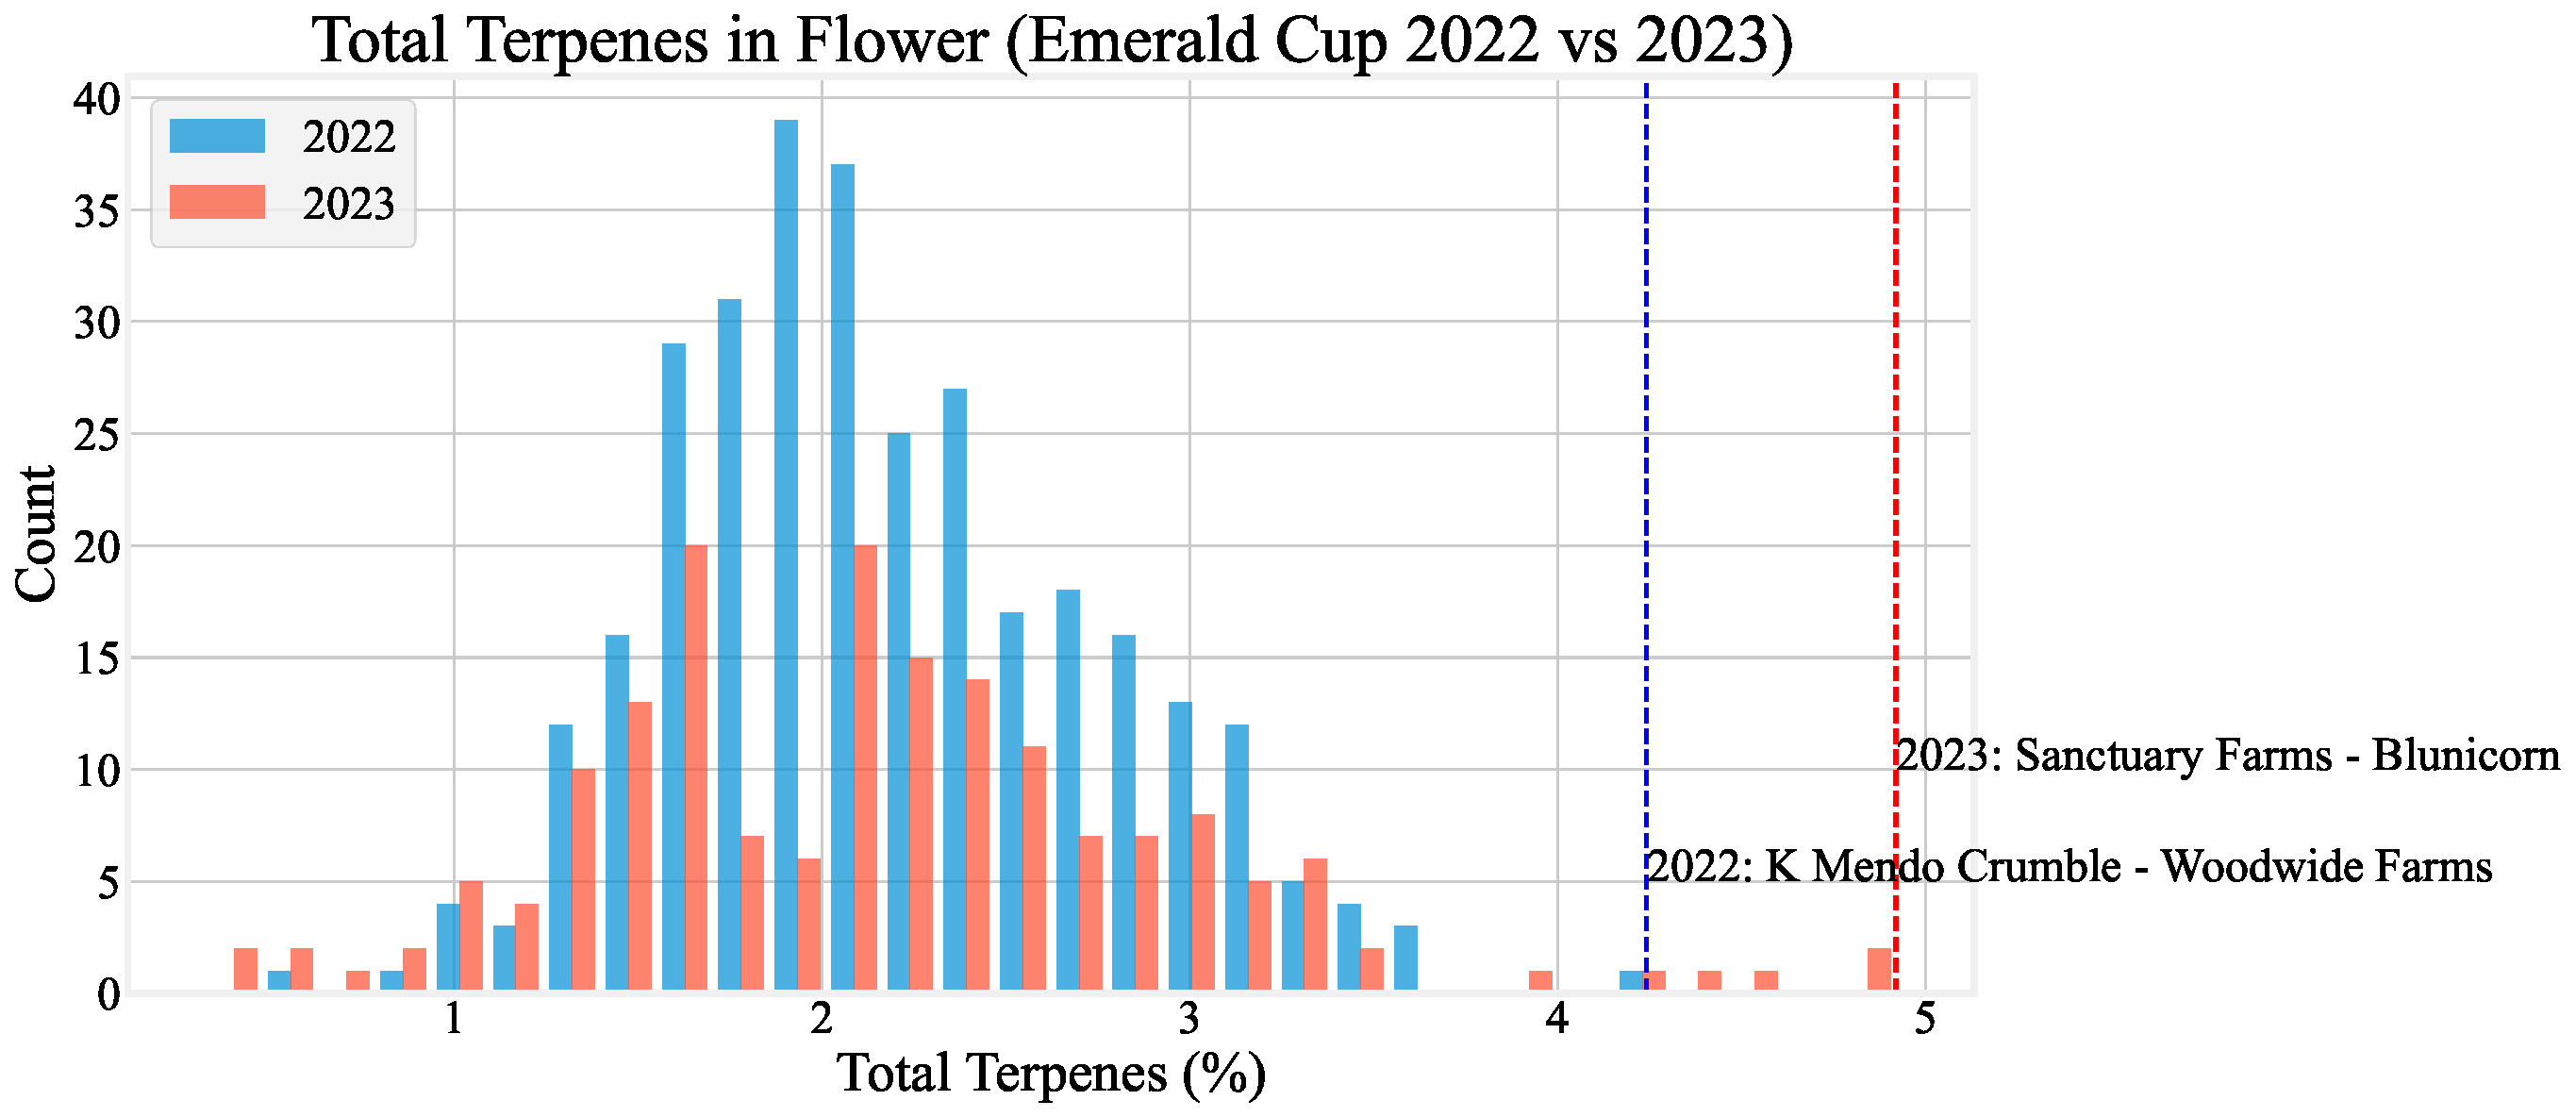
\includegraphics[width=0.8\textwidth]{images/emerald-cup-total-terpenes-histogram.pdf}
\end{center}

\end{frame}


%------------------------------------------%
% Chemical Diversity
%------------------------------------------%

\begin{frame}{Chemical Diversity}

\begin{minipage}{0.5\textwidth}
    \scriptsize
    \includegraphics[width=0.65\linewidth]{images/claude-shannon.jpg}\\
    \textbf{Claude Shannon} (1916 - 2001)\\
    The father of information theory.
\end{minipage}%
\begin{minipage}{0.5\textwidth}
\footnotesize

{\bfseries The Shannon Diversity Index}, $H'$, is a commonly used measure of diversity.

$$
H' = -\sum_{i=1}^{s} p_i \ln(p_i).
$$

\scriptsize
Note:\\[0.5em]
\begin{itemize}
\item $s$ represents the total number of species in the dataset.\\[1em]
\item $p_i$ is the proportion of individuals belonging to the $i$-th species in the dataset.\\[1em]
\item A higher value of $H'$ indicates greater diversity.
\end{itemize}

\end{minipage}


\end{frame}


%------------------------------------------%
% Terpene Diversity
%------------------------------------------%

% Official winners
\begin{frame}{Most Unique Terpene Profile Official Winners}

\vspace{0.5\baselineskip}

\begin{minipage}{0.5\textwidth}
    \scriptsize
    \includegraphics[width=0.5\linewidth]{images/juice-z.png}\\
    \textbf{2022:} Juice Z\\
    by Atrium Cultivation\\
    \textit{Terpene diversity: 3.19}
\end{minipage}%
\begin{minipage}{0.5\textwidth}
\footnotesize
\includegraphics[width=0.5\textwidth]{images/lilac-mintz.png}\\
\textbf{2023:} Lilac Mintz\\
by Healing Herb Farms\\
\textit{Terpene diversity: 3.03}
\end{minipage}

% Terpene diversity histogram
\vspace{5pt}
\begin{center}
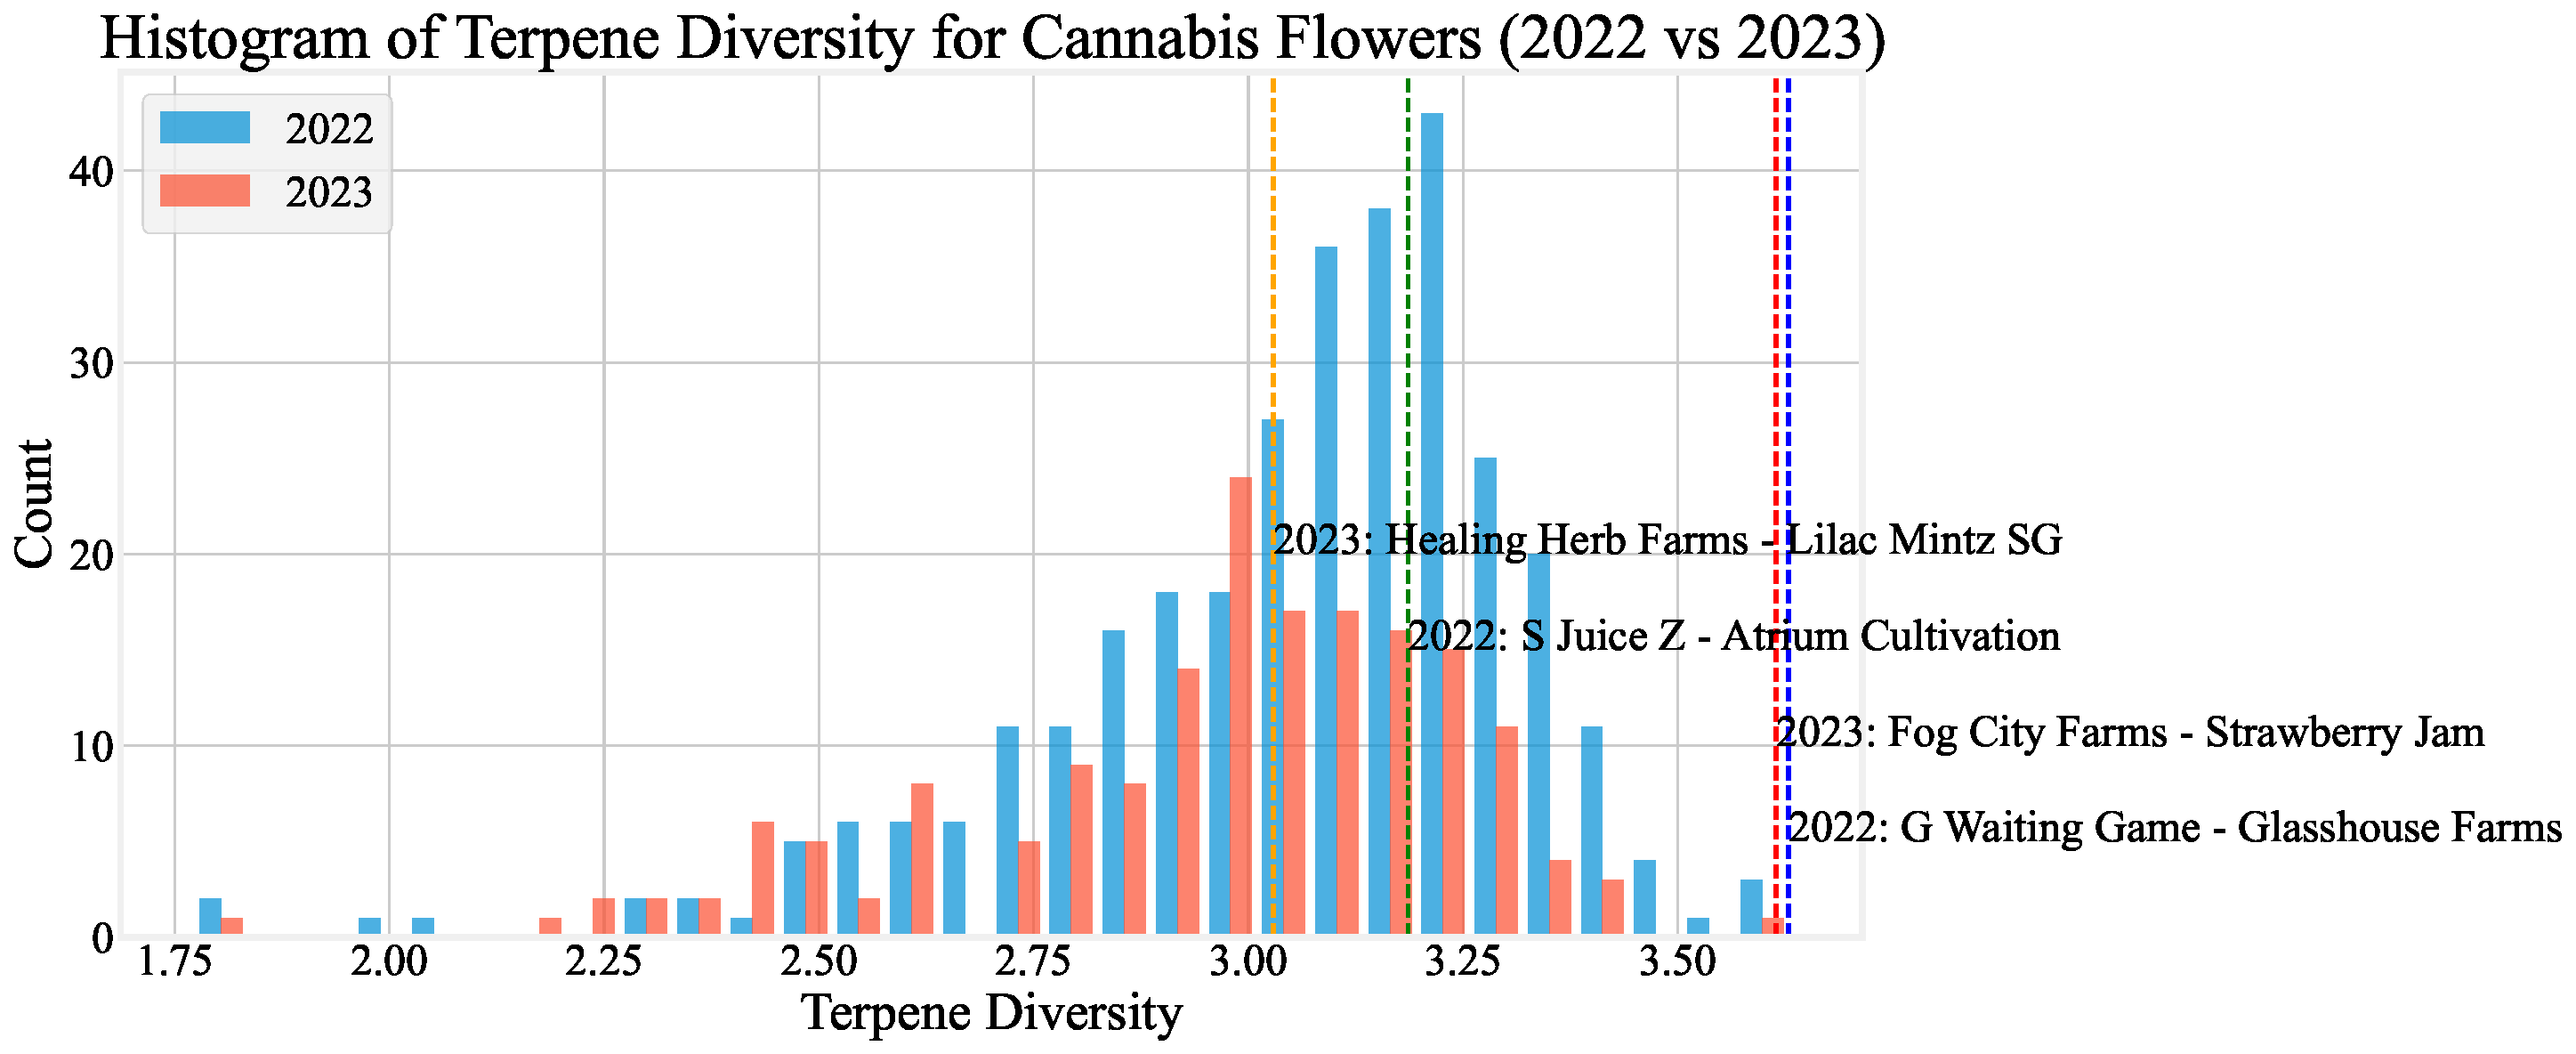
\includegraphics[width=0.9\textwidth]{images/emerald-cup-terpene-diversity-histogram.pdf}
\end{center}

\end{frame}


%------------------------------------------%
% Terpene Profiles
%------------------------------------------%

% Predicted winners
\begin{frame}{Highest Terpene Diversity}

  \begin{minipage}{0.5\textwidth}
    \scriptsize
    \includegraphics[width=0.5\linewidth]{images/waiting-game.png}\\
    \textbf{2022:} Waiting Game\\
    by Glasshouse Farms\\
    \textit{Terpene diversity: 3.63}
\end{minipage}%
\begin{minipage}{0.5\textwidth}
\footnotesize
\includegraphics[width=0.5\textwidth]{images/strawberry-jam.png}\\
\textbf{2023:} Strawberry Jam\\
by Fog City Farms\\
\textit{Terpene diversity: 3.61}
\end{minipage}

  % Terpene diversity barchart
  \vspace{10pt}
  \begin{center}
  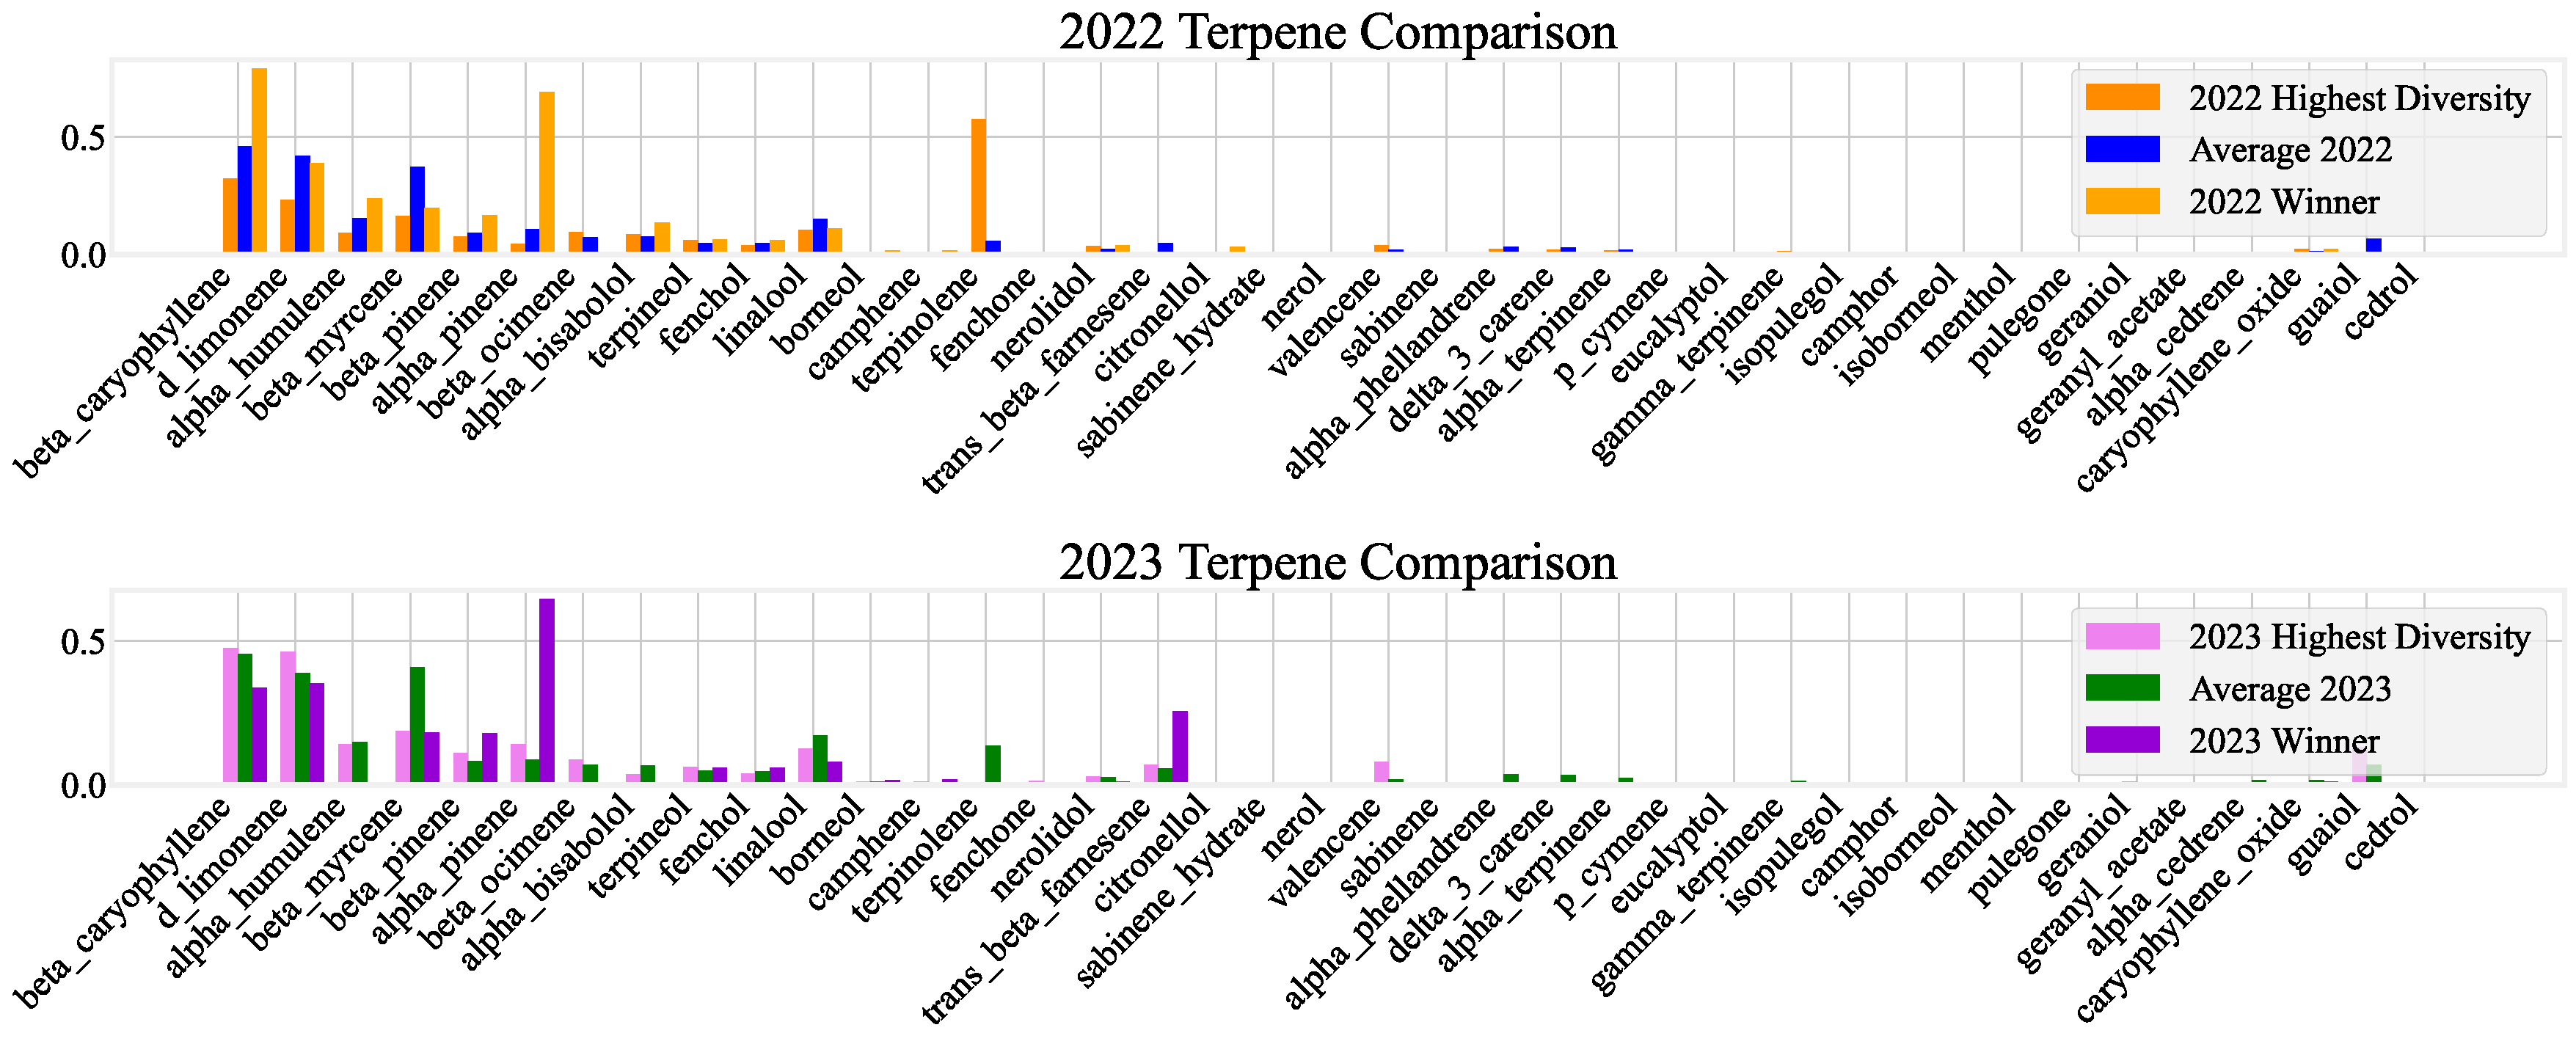
\includegraphics[width=\textwidth]{images/emerald-cup-terpene-diversity-winner.pdf}
  \end{center}
  
\end{frame}


%------------------------------------------%
% Cannabinoid Diversity
%------------------------------------------%

\begin{frame}{Most Unique Cannabinoid Profile}

% FIXME:
\begin{minipage}{0.33\textwidth}
    \footnotesize
    \textbf{2022 \nth{2} place}\\
    Mendo Purps\\
    by Lempire Farmaseed\\
    \begin{figure}[H]
        \centering
        \includegraphics[width=0.7\linewidth]{images/mendo-purps.png}
    \end{figure}
\end{minipage}%
\begin{minipage}{0.33\textwidth}
    \footnotesize
    \textbf{2023 \nth{2} place}\\
    Joyful \& Present PR\\
    by Garden Society\\
    \begin{figure}[H]
        \centering
        \includegraphics[width=0.7\linewidth]{images/joyful-and-present.png}
    \end{figure}
\end{minipage}%
\begin{minipage}{0.33\textwidth}
    \footnotesize
    \textbf{2022 and 2023 winner}\\
    Pink Boost Goddess\\
    by Emerald Spirit Botanicals\\
    \begin{figure}[H]
        \centering
        \includegraphics[width=0.7\linewidth]{images/pink-boost-goddess.png}
    \end{figure}
\end{minipage}

  % Cannabinoid diversity histogram.
  \centering
  \vspace{10pt}
  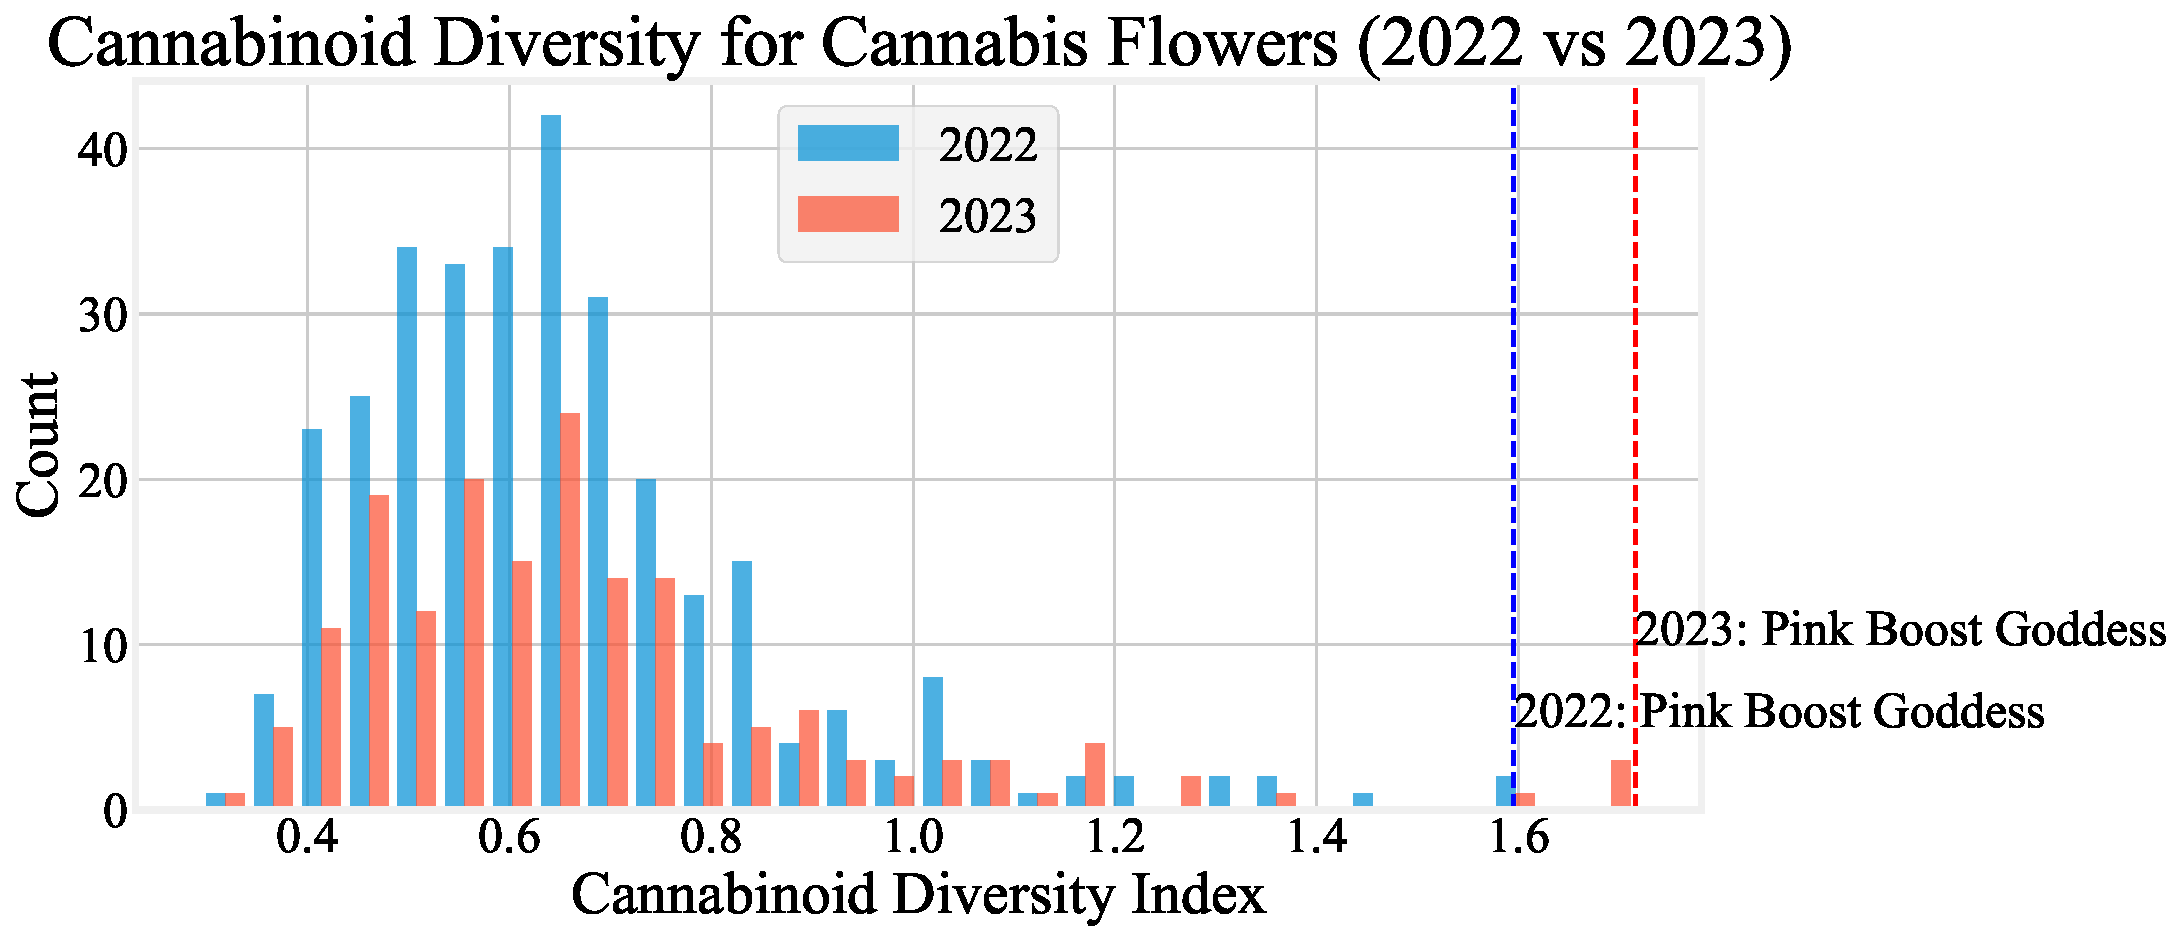
\includegraphics[width=0.8\textwidth]{images/emerald-cup-cannabinoid-diversity-histogram.pdf}

\end{frame}



% Slide for Cannabinoid diversity winner
\begin{frame}{Cannabinoid Diversity}

  \centering
  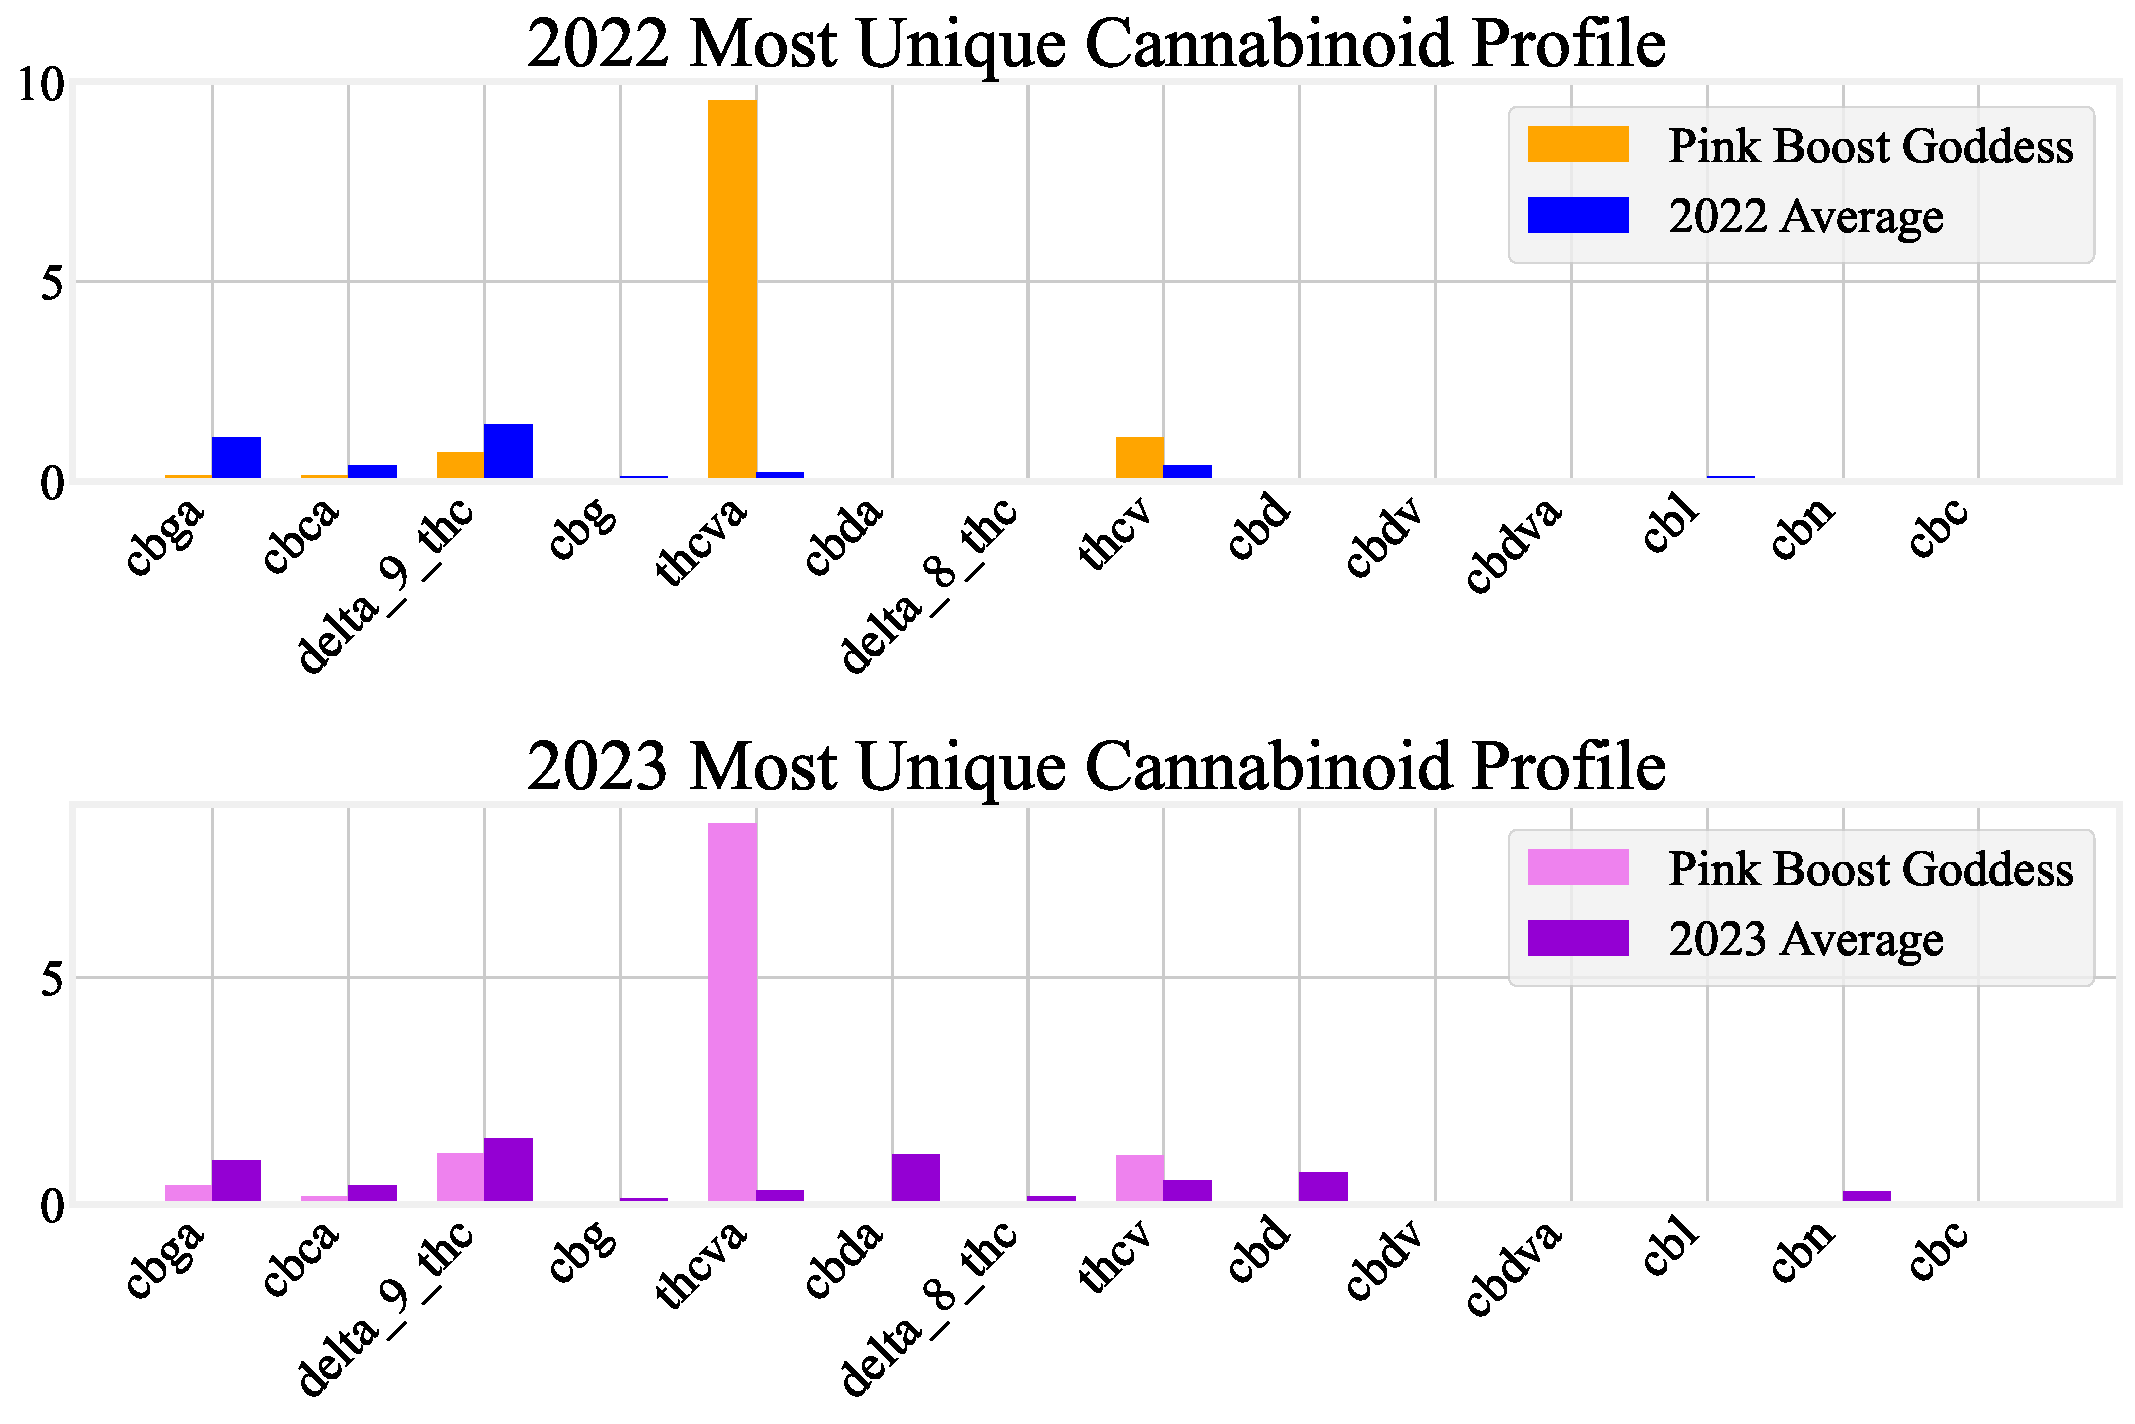
\includegraphics[width=\textwidth]{images/emerald-cup-cannabinoid-diversity-winner.pdf}
\end{frame}


%------------------------------------------%
% Colorimetry
%------------------------------------------%

\begin{frame}{Colorimetry}

{\footnotesize Early colorimetry was concerned with the specification of color in terms of the human eye's response to \textbf{\textcolor{red}{red}}, \textbf{\textcolor{green}{green}}, and \textbf{\textcolor{blue}{blue}} light.\\}

\vspace{1.5\baselineskip}

\begin{columns}

\column{0.5\textwidth}
\centering
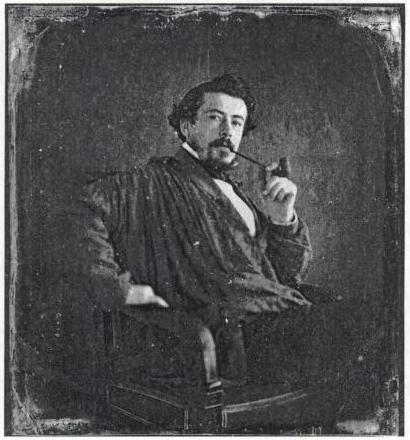
\includegraphics[width=0.9\linewidth]{images/duboscq-jules.jpg}\\
\scriptsize{\textbf{Louis Jules Dubosq} (1817 - 1886)\\
Inventor of an early colorimeter.}

\column{0.5\textwidth}

\begin{center}
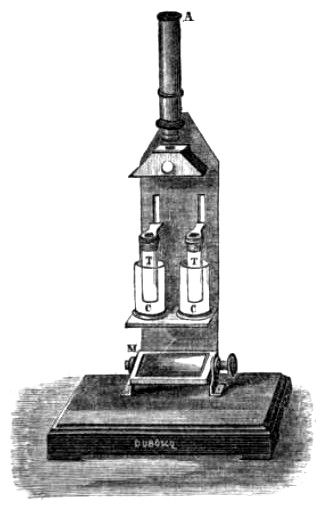
\includegraphics[width=0.5\linewidth]{images/duboscq-colorimeter-1870.jpg}
\end{center}
\scriptsize{Drawing of one of the first {\bfseries colorimeters}, built by Jules Duboscq in France.}

\end{columns}
\end{frame}


\begin{frame}{Colourfulness - A modern day metric of color}


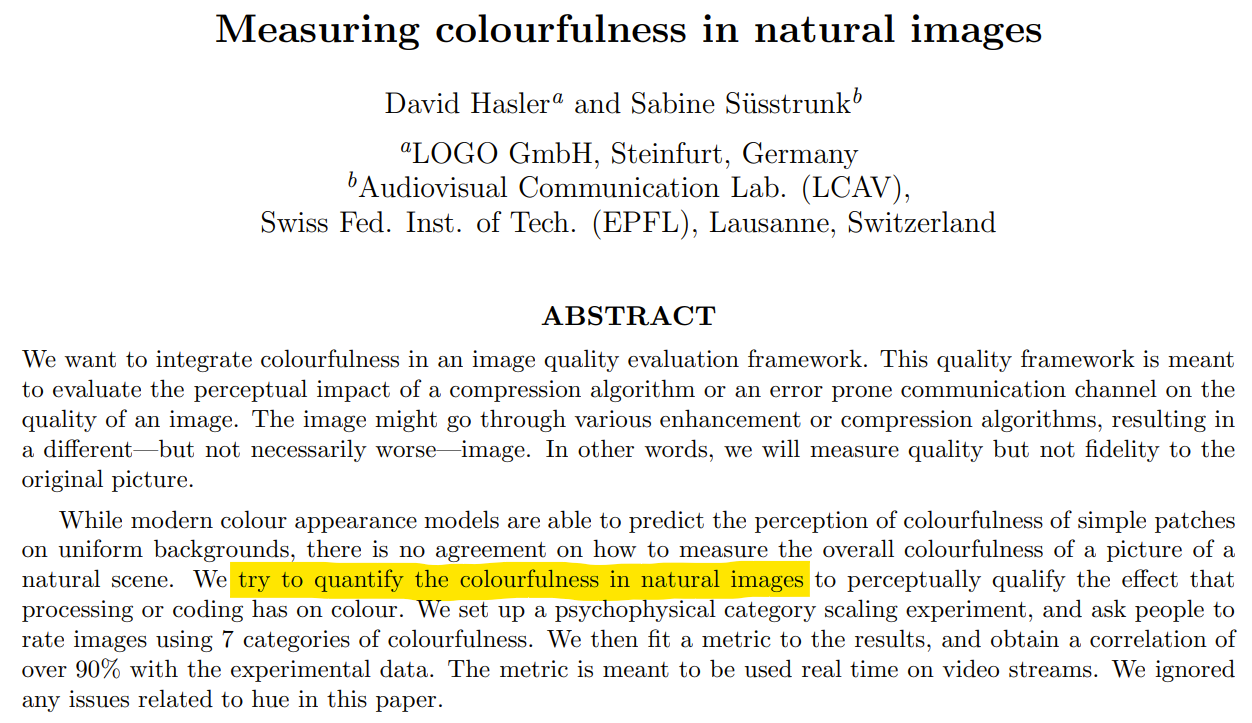
\includegraphics[width=\linewidth]{images/colourfulness-abstract.png}

\vfill
{\tiny Source: Hasler, David \& Suesstrunk, Sabine. (2003). Measuring Colourfulness in Natural Images. Proceedings of SPIE - The International Society for Optical Engineering. \\http://dx.doi.org/10.1117/12.477378}

\end{frame}

\begin{frame}{Colourfulness - A modern day metric of color}

\includegraphics[width=\linewidth]{images/colourfulness-definition.png}

\begin{center}
\includegraphics[width=0.25\linewidth]{images/colourfulness-definition-2.png}
\end{center}

\vfill
{\tiny Source: Hasler, David \& Suesstrunk, Sabine. (2003). Measuring Colourfulness in Natural Images. Proceedings of SPIE - The International Society for Optical Engineering. \\http://dx.doi.org/10.1117/12.477378}


\end{frame}


%------------------------------------------%
% Most Colorful
%------------------------------------------%


\begin{frame}{Cannlytics Most Colorful Flower Award}

\vspace{\baselineskip}

  % Most Colorful Flower
\begin{minipage}{0.5\textwidth}
    \footnotesize
    \textbf{2022 Most Colorful Flower}\\
    Rainbow Beltz\\
    by Royal Bloodline
    \begin{figure}[H]
        \centering
        \includegraphics[width=0.5\linewidth]{images/rainbow-beltz.png}
    \end{figure}
\end{minipage}%
\begin{minipage}{0.5\textwidth}
    \footnotesize
    \textbf{2023 Most Colorful Flower}\\
    Orange Creampop 38\\
    Burr's Place
    \begin{figure}[H]
        \centering
        \includegraphics[width=0.5\linewidth]{images/orange-creampop.png}
    \end{figure}
\end{minipage}

  \centering
  \vspace{10pt}
  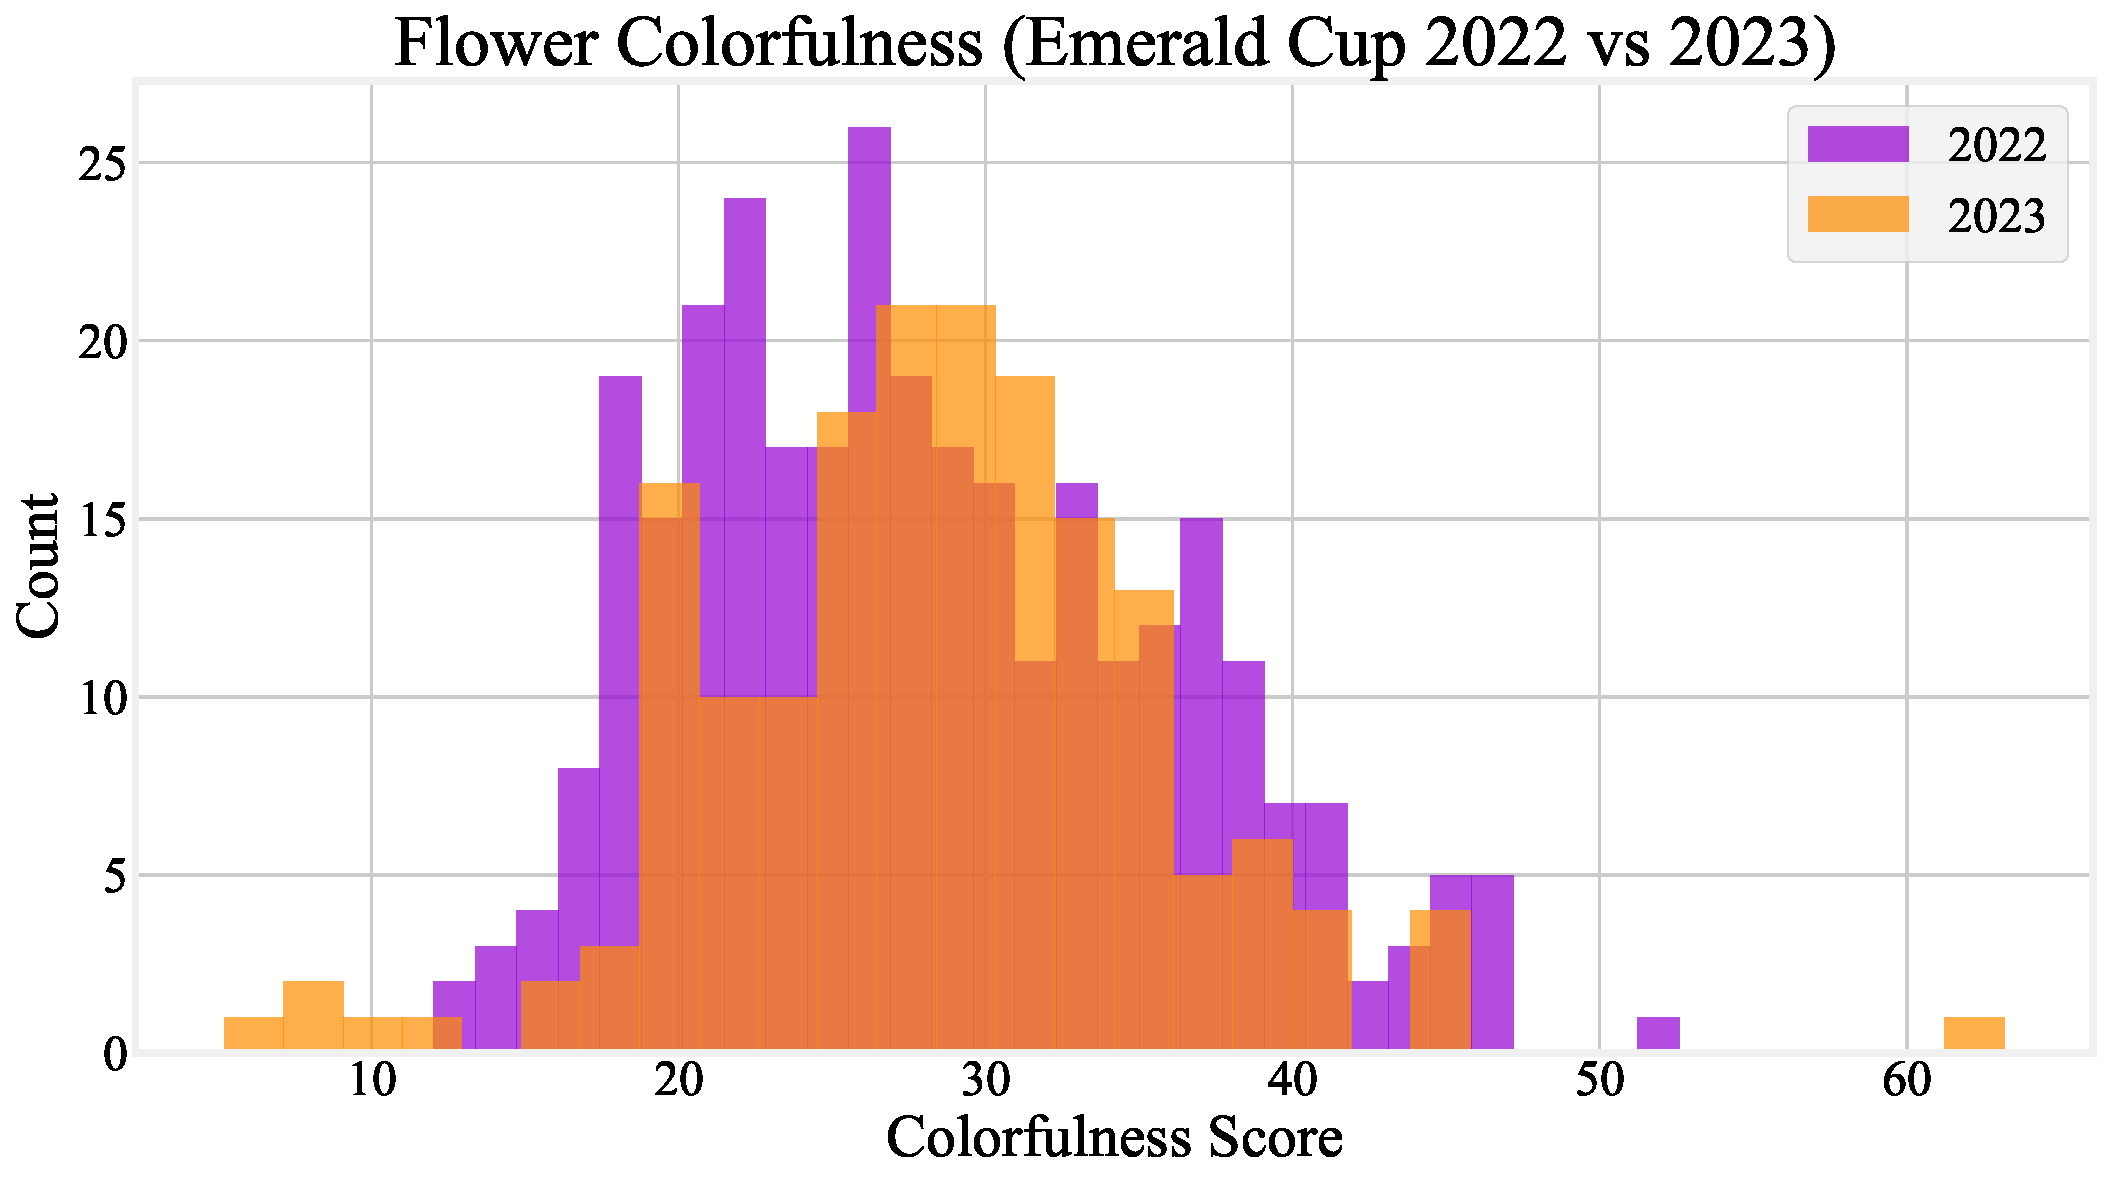
\includegraphics[width=0.8\textwidth]{images/emerald-cup-colorfulness-scores.pdf}
  
\end{frame}


%------------------------------------------%
% Top 10 Most Colorful Strains
%------------------------------------------%

\begin{frame}{Top 5 Most Colorful Strains - 2022}
\scriptsize

\begin{tabular}{lcL{4cm}r}
\toprule
Image & Rank & Product Name & Colorfulness Score \\
\midrule
\includegraphics[width=0.15\textwidth]{images/220224Q048.png} & 1 & K Rainbow Beltz - Royal Bloodline & 52.58 \\
\includegraphics[width=0.15\textwidth]{images/220224Q039.png} & 2 & P Summer Punch - Panos Bogiantzis & 46.89 \\
\includegraphics[width=0.15\textwidth]{images/220301Q046.png} & 3 & S Jelly Runtz - Humboldt Seed Company & 46.63 \\
\includegraphics[width=0.15\textwidth]{images/220224Q032.png} & 4 & P 3 Kings - Jon Kelly & 46.27 \\
\includegraphics[width=0.15\textwidth]{images/220307S046.png} & 5 & G Orange Pop - SoHum Royal & 46.05 \\
\bottomrule
\end{tabular}

\end{frame}

\begin{frame}{Top 5 Most Colorful Strains - 2023}
\scriptsize

\begin{tabular}{lcL{4cm}r}
\toprule
Image & Rank & Product Name & Colorfulness Score \\
\midrule
\includegraphics[width=0.15\textwidth]{images/230314U025.png} & 1 & Emerald Spirit Botanicls - Pink Boost Goddess 3S & 45.37 \\
\includegraphics[width=0.15\textwidth]{images/230314U025.png} & 2 & Emerald Spirit Botanicls - Pink Boost Goddess 3S & 45.37 \\
\includegraphics[width=0.15\textwidth]{images/230311S009.png} & 3 & Burr's Place - Orange Creampop 38 & 44.82 \\
\includegraphics[width=0.15\textwidth]{images/230217R028.png} & 4 & Panos Bogiantzis - Nfsheeeesh & 41.33 \\
\includegraphics[width=0.15\textwidth]{images/230217R027.png} & 5 & Panos Bogiantzis - Tropical Purple Kush & 41.25 \\
\bottomrule
\end{tabular}

\end{frame}


%------------------------------------------%
% Definition of Purple
%------------------------------------------%

\begin{frame}{The Color Purple}

{\footnotesize
Define a {\bfseries purpleness function} that calculates a value based on the intensities of the red (R), green (G), and blue (B) color channels in the RGB color model, with each channel ranging from 0 to 255.}

$$
\text{Purpleness} \equiv (R + B) - 2 \times G
$$


\vspace{1\baselineskip}
{\scriptsize {\bfseries Maxiumum purple} occurs when $R = B = 255$ and $G = 0$.\\
$$
\text{Max Purpleness} = (255 + 255) - 2 \times 0 = 510
$$
\definecolor{purepurple}{RGB}{255, 0, 255}
\begin{center}
\colorbox{purepurple}{\hspace{1cm} \phantom{Pure Purple} \hspace{1cm}}\\
\end{center}
}

{\scriptsize

\vspace{2\baselineskip}
\textbf{Minimum Purple} occurs when $R = B = 0$ and $G = 255$.\\
$$
\text{Min Purpleness} = (0 + 0) - 2 \times 255 = -510
$$
\definecolor{purepurple}{RGB}{0, 255, 0}
\begin{center}
\colorbox{purepurple}{\hspace{1cm} \phantom{Pure Purple} \hspace{1cm}}\\
\end{center}
}

% Put a patch of pure purple
\end{frame}


%------------------------------------------%
% Most Purple
%------------------------------------------%

\begin{frame}{Cannlytics Most Purple Flower Award}

\vspace{\baselineskip}

% Most Purple Flower
\begin{minipage}{0.5\textwidth}
    \scriptsize
    \textbf{2022 Most Purple Flower}\\
    Silver Squatch\\
    by Paula Jobe
    \begin{figure}[H]
        \centering
        \includegraphics[width=0.5\linewidth]{images/silver-squatch.png}
    \end{figure}
\end{minipage}%
\begin{minipage}{0.5\textwidth}
    \scriptsize
    \textbf{2023 Most Purple Flower}\\
    Blue Meringue Hemp\\
    by Flow Gardens
    \begin{figure}[H]
        \centering
        \includegraphics[width=0.5\linewidth]{images/blue-meringue.png}
    \end{figure}
\end{minipage}

  \centering
  \vspace{10pt}
  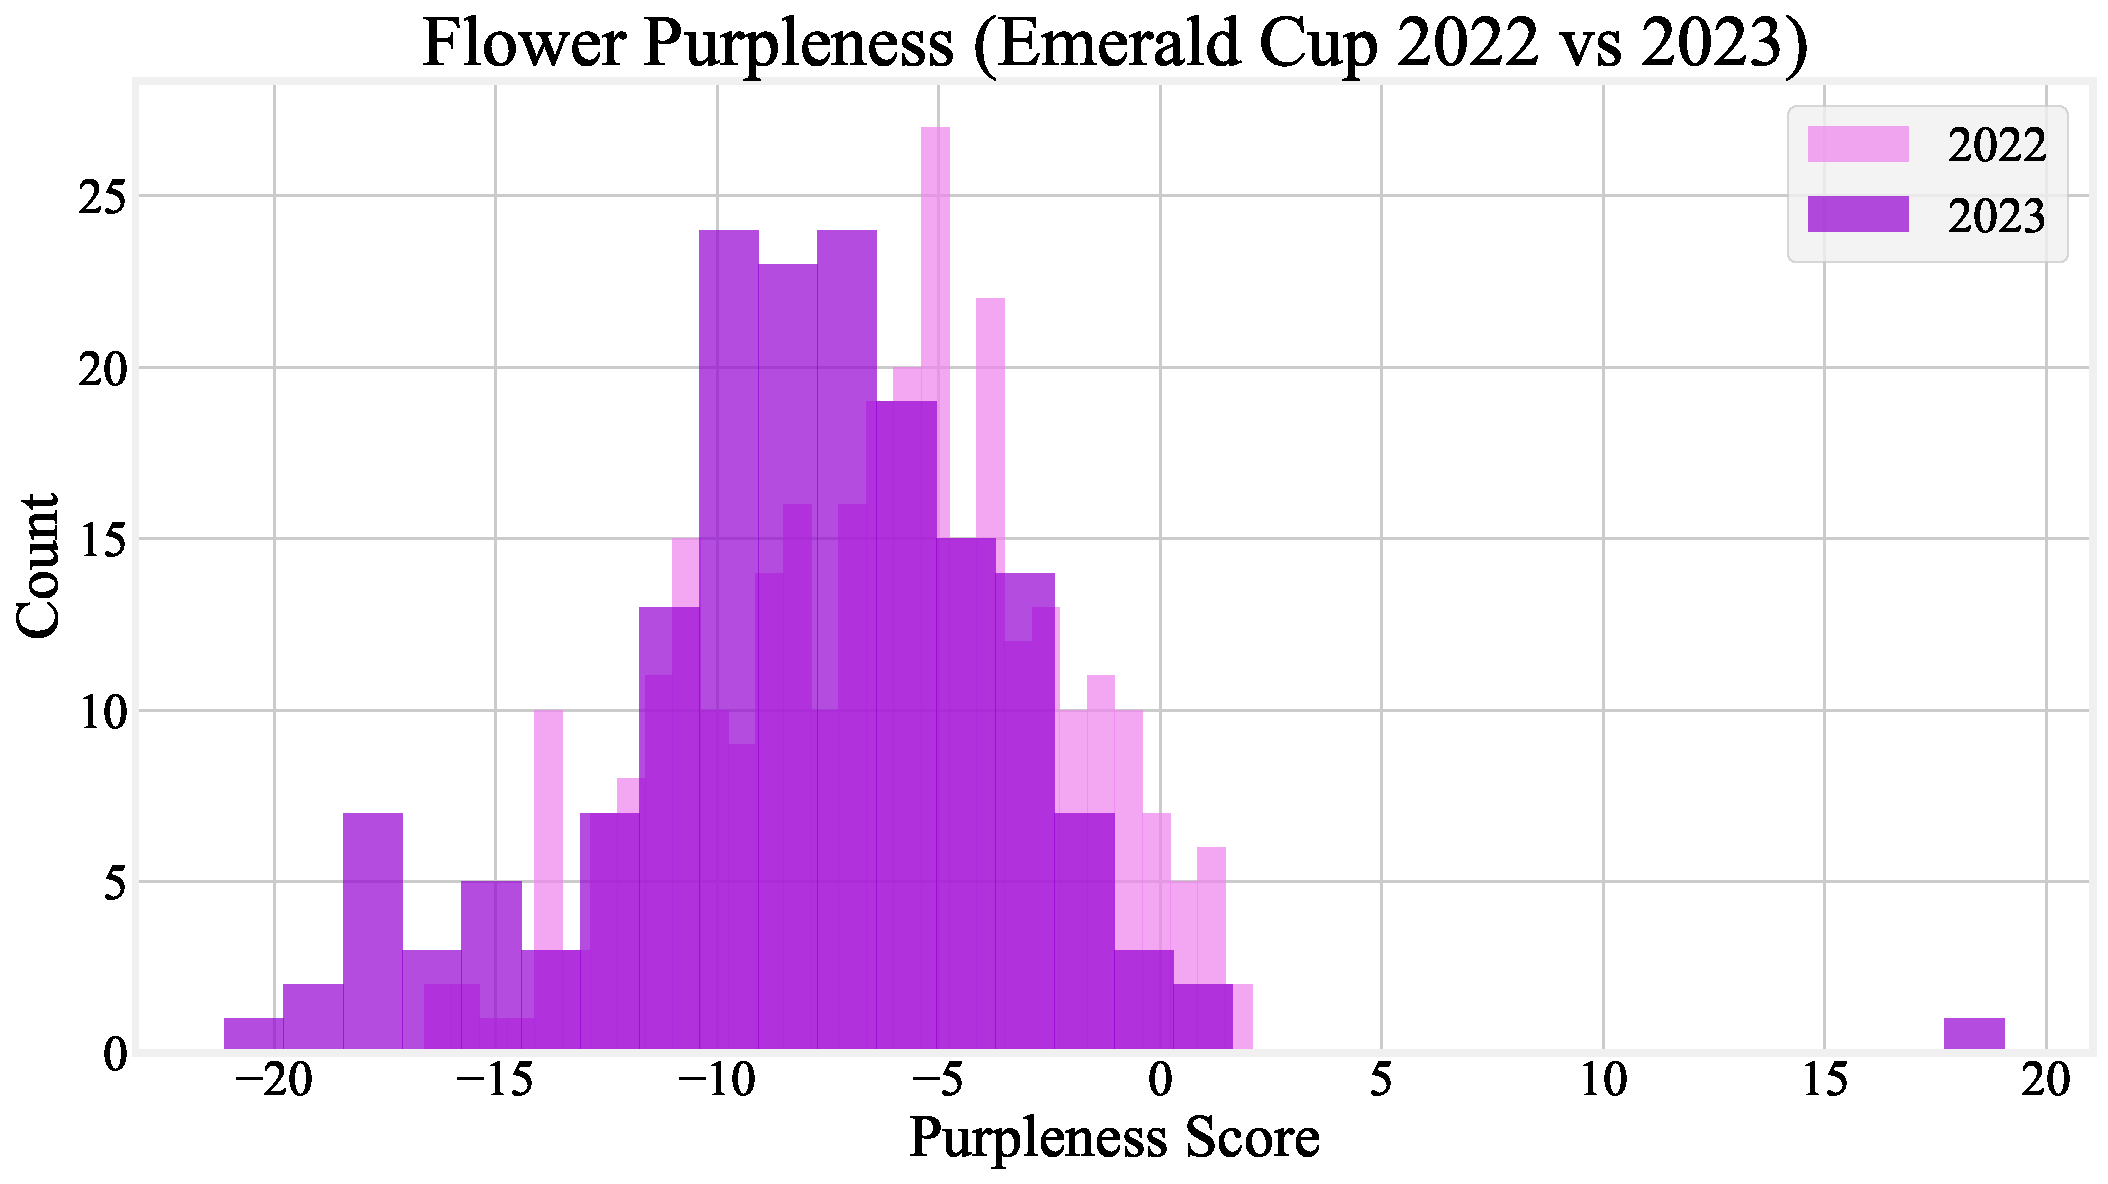
\includegraphics[width=0.8\textwidth]{images/emerald-cup-purple-scores.pdf}
  

\end{frame}

%------------------------------------------%
% Top 10 Most Purple Strains
%------------------------------------------%


\begin{frame}{Top 5 Most Purple Strains - 2022}
\scriptsize

\begin{tabular}{lcL{4cm}r}
\toprule
Image & Rank & Product Name & Purpleness \\
\midrule
\includegraphics[width=0.15\textwidth]{images/220303R035.png} & 1 & P Silver Squatch - Paula Jobe & 2.09 \\
\includegraphics[width=0.15\textwidth]{images/220228R046.png} & 2 & S \#26 - Canna Country Farm & 1.50 \\
\includegraphics[width=0.15\textwidth]{images/220304S048.png} & 3 & K Biscotti - Connected Cannabis & 1.28 \\
\includegraphics[width=0.15\textwidth]{images/220303R057.png} & 4 & S Pink Jesus Flower - Sonoma Hill Farms & 1.10 \\
\includegraphics[width=0.15\textwidth]{images/220304S045.png} & 5 & K Slow Lane - Connected & 0.99 \\
\bottomrule
\end{tabular}

\end{frame}

\begin{frame}{Top 5 Most Purple Strains - 2023}
\scriptsize

\begin{tabular}{lcL{4cm}r}
\toprule
Image & Rank & Product Name & Purpleness \\
\midrule
\includegraphics[width=0.15\textwidth]{images/230316R009.png} & 0 & Local Cannabis Co - ICC Badder PR & 19.05 \\
\includegraphics[width=0.15\textwidth]{images/230316U006.png} & 1 & Flow Gardens - Blue Meringue Hemp & 0.59 \\
\includegraphics[width=0.15\textwidth]{images/230311S046.png} & 2 & STIIIZY - Gelato Runtz & 0.46 \\
\includegraphics[width=0.15\textwidth]{images/230313S007.png} & 3 & Humboldt Gardens - Gelly Runtz I & 0.19 \\
\includegraphics[width=0.15\textwidth]{images/230311S042.png} & 4 & Pure Beauty - Mendo Breath & -0.22 \\
\includegraphics[width=0.15\textwidth]{images/230316U001.png} & 5 & Hemp Hop - Abacus Diesel Hemp & -0.84 \\
\bottomrule
\end{tabular}

\end{frame}


%------------------------------------------%
% Most Green
%------------------------------------------%

\begin{frame}{Cannlytics Green Green Award}

\vspace{\baselineskip}

% Most Green Flower
\begin{minipage}{0.5\textwidth}
    \scriptsize
    \textbf{2022 Most Green Flower}\\
    Jelly Runtz\\
    by Humboldt Seed Company
    \begin{figure}[H]
        \centering
        \includegraphics[width=0.5\linewidth]{images/jelly-runtz.png}
    \end{figure}
\end{minipage}%
\begin{minipage}{0.5\textwidth}
    \scriptsize
    \textbf{2023 Most Green Flower}\\
    Double OG Chem\\
    by Colin Teurfs
    \begin{figure}[H]
        \centering
        \includegraphics[width=0.5\linewidth]{images/double-og-chem.png}
    \end{figure}
\end{minipage}

  \centering
  \vspace{10pt}
  \includegraphics[width=0.8\textwidth]{images/emerald-cup-greenness-scores.pdf}

\end{frame}

%------------------------------------------%
% Top 10 Most Green Strains
%------------------------------------------%

\begin{frame}{Top 5 Most Green Strains - 2022}
\scriptsize

\begin{tabular}{lcL{4cm}r}
\toprule
Image & Rank & Product Name & Greenness \\
\midrule
\includegraphics[width=0.15\textwidth]{images/220301Q046.png} & 1 & S Jelly Runtz - Humboldt Seed Company & -16.61 \\
\includegraphics[width=0.15\textwidth]{images/220224Q033.png} & 2 & P Mimosa \#3 - Andrew Leitch & -16.21 \\
\includegraphics[width=0.15\textwidth]{images/220224Q048.png} & 3 & K Rainbow Beltz - Royal Bloodline & -15.96 \\
\includegraphics[width=0.15\textwidth]{images/220224Q060.png} & 4 & M Lemon Royale - Talking Trees Farms & -15.80 \\
\includegraphics[width=0.15\textwidth]{images/220307S046.png} & 5 & G Orange Pop - SoHum Royal & -14.90 \\
\bottomrule
\end{tabular}

\end{frame}

\begin{frame}{Top 5 Most Green Strains - 2023}
\scriptsize

\begin{tabular}{lcL{4cm}r}
\toprule
Image & Rank & Product Name & Greenness \\
\midrule
\includegraphics[width=0.15\textwidth]{images/230217R029.png} & 1 & Colin Teurfs - Double OG Chem SG & -21.12 \\
\includegraphics[width=0.15\textwidth]{images/230314U002.png} & 2 & CannaCruz - Blackberry Cream I & -19.39 \\
\includegraphics[width=0.15\textwidth]{images/230314U004.png} & 3 & CannaCruz - Biscotti-otti-otti I & -19.14 \\
\includegraphics[width=0.15\textwidth]{images/230314U003.png} & 4 & CannaCruz - Lemon Cherry Gelato I & -18.30 \\
\includegraphics[width=0.15\textwidth]{images/230217R027.png} & 5 & Panos Bogiantzis - Tropical Purple Kush & -18.06 \\
\bottomrule
\end{tabular}

\end{frame}




%------------------------------------------%
% Ordinal Probit Model
%------------------------------------------%

\begin{frame}{Challenge: Predict Emerald Cup 2024 Winners!}
\scriptsize

\vspace{0.5\baselineskip}
The {\bfseries ordered probit model} can be used to estimate relationships for categorical data. Consider:

\[ y^* = \mathbf{x}^{\mathsf{T}} \beta + \epsilon \]

\vspace{-0.5\baselineskip}
Where:
\vspace{0.5\baselineskip}

\begin{itemize}
    \item $y^*$ is the {\itshape exact} but \underline{unobserved} dependent variable.
    \item $\mathbf{x}$ is the vector of independent variables.
    \item $\beta$ is the vector of regression coefficients.
\end{itemize}

\vspace{1\baselineskip}
However, we observe categories, $y$:
\[ 
y= \begin{cases}
0~~ \text{if}~~y^* \le 0, \\
1~~ \text{if}~~0<y^* \le \mu_1, \\
\vdots \\
N~~ \text{if}~~ \mu_{N-1} < y^*.
\end{cases}
\]

The {\bfseries ordered probit} uses observations, $\mathbf{x}$ and $y$, to estimate the parameters, $\hat{\beta}$.

\end{frame}




%------------------------------------------%
% Takeaway
%------------------------------------------%
\section{Takeaway}
\begin{frame}{}

\begin{center}
\begin{minipage}{3.85in}

% Thank you.
\includegraphics[width=.25in]{images/prayer.png} {\Large \textbf{Thank you for coming.}}\\

% Re-cap the lesson of the week.
\begin{center}
\begin{minipage}{\linewidth}
\begin{Block}{Lessons of the Day}

\vspace{\baselineskip}

\begin{itemize}

\item The grass is always \textcolor{OliveGreen}{\bfseries greener} on the other side.

\vspace{\baselineskip}

\item Sometimes, playing the \textcolor{OliveGreen}{\bfseries waiting game} works so well others don't realize how far ahead you are!

\vspace{\baselineskip}

\end{itemize}

\end{Block}
\end{minipage}
\end{center}

\vfill

\end{minipage}
\end{center}

\end{frame}


%------------------------------------------%
% End
%------------------------------------------%
\end{document}
